\tikzstyle{startstop} = [rectangle, rounded corners, minimum width=10cm, minimum height=1.5cm,text centered, draw=black, fill=green!20]
\begin{center}
	\begin{tikzpicture}
		\node (start) [startstop] {\bfseries \text{ÔN TẬP TUẦN 4}};
	\end{tikzpicture}
\end{center}
\setcounter{section}{0}
\Opensolutionfile{ans}[ans/G10TUAN4-TN]
% ===================================================================
\begin{ex}
	Chọn đáp án có từ /cụm từ thích hợp để hoàn thành bảng sau:
	\begin{center}
		\begin{tabular}{|c|c|c|}
			\hline
			\bfseries Đơn vị &\bfseries Kí hiệu & \bfseries Đại lượng\\
			\hline
			kelvin & (1) & (2)\\
			\hline
			ampe & $\si{\ampere}$ & (3)\\
			\hline
			candela & $\si{\candela}$ & (4)\\
			\hline
		\end{tabular}
	\end{center}
	\choice
	{(1) $\si{\kelvin}$; (2) Khối lượng; (3) Cường độ dòng điện; (4) Lượng chất}
	{\True (1) $\si{\kelvin}$; (2) Nhiệt độ; (3) Cường độ dòng điện; (4) Cường độ ánh sáng}
	{(1) $\si{\kelvin}$; (2) Nhiệt độ; (3) Cường độ dòng điện; (4) Lượng chất}
	{(1) $\si{\kelvin}$; (2) Khối lượng; (3) Cường độ dòng điện; (4) Cường độ ánh sáng}
	\loigiai{}
\end{ex}
% ===================================================================
\begin{ex}
	Đơn vị nào sau đây không thuộc thứ nguyên $L$ [Chiều dài]?
	\choice
	{Dặm}
	{Hải lí}
	{Năm ánh sáng}
	{\True Năm}
	\loigiai{}
\end{ex}
% ===================================================================
\begin{ex}
Đáp án nào sau đây có 1 đơn vị cơ bản và 1 đơn vị dẫn xuất?	
	\choice
	{mét, kilogram}
	{\True newton, mol}
	{pascal, joule}
	{candela, kelvin}
	\loigiai{}
\end{ex}
% ===================================================================
\begin{ex}
	Hãy chọn câu phát biểu \textbf{đúng}?
	\choice
	{Hệ quy chiếu bao gồm hệ toạ độ, mốc thời gian và đồng hồ}
	{Hệ quy chiếu bao gồm vật làm mốc, mốc thời gian và đồng hồ}
	{Hệ quy chiếu bao gồm vật làm mốc, hệ toạ độ, mốc thời gian}
	{\True Hệ quy chiếu bao gồm vật làm mốc, hệ toạ độ, mốc thời gian và đồng hồ}
	\loigiai{}
\end{ex}
% ===================================================================
\begin{ex}
Kết luận nào sau đây là \textbf{đúng} khi nói về độ dịch chuyển và quãng đường đi được của một vật?	
	\choice
	{Độ dịch chuyển và quãng đường đi được đều là đại lượng vô hướng}
	{\True Độ dịch chuyển là đại lượng vector còn quãng đường đi được là đại lượng vô hướng}
	{Độ dịch chuyển và quãng đường đi được đều là đại lượng vector}
	{Độ dịch chuyển và quãng đường đi được đều là đại lượng không âm}
	\loigiai{}
\end{ex}
% ===================================================================
\begin{ex}
	Khi vật chuyển động thẳng đều cùng chiều dương thì đồ thị $d - t$ của vật có dạng là
	\choice
	{đường thẳng vuông góc với trục $Od$}
	{\True đường thẳng xiên góc đi lên}
	{đường thẳng xiên góc đi xuống}
	{đường thẳng vuông góc với trục $Ot$}
	\loigiai{}
\end{ex}
% ===================================================================
\begin{ex}
	Cho đồ thị độ dịch chuyển – thời gian của một vật như hình. Chọn phát biểu \textbf{đúng}.	
	\begin{center}
		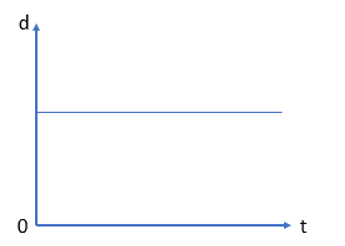
\includegraphics[width=0.25\linewidth]{figs/VN10-2023-PH-TP005-P-1}
	\end{center}
	\choice
	{Vật đang chuyển động thẳng đều theo chiều dương}
	{Vật đang chuyển động thẳng đều theo chiều âm}
	{\True Vật đang đứng yên}
	{Vật chuyển động thẳng đều theo chiều dương rồi đổi chiều chuyển động ngược lại}
	\loigiai{}
\end{ex}

% ===================================================================
\begin{ex}
Một vật bắt đầu chuyển động từ điểm O đến điểm A, sau đó chuyển động về điểm B. Quãng đường và độ dịch chuyển của vật tương ứng là	
\begin{center}
	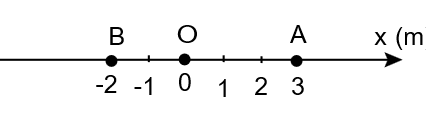
\includegraphics[width=0.4\linewidth]{figs/VN10-2022-PH-TP004-P-2}
\end{center}
	\choice
	{$\SI{2}{\meter}$; $\SI{-2}{\meter}$}
	{\True $\SI{8}{\meter}$; $\SI{-2}{\meter}$}
	{$\SI{2}{\meter}$; $\SI{2}{\meter}$}
	{$\SI{8}{\meter}$; $\SI{-8}{\meter}$}
	\loigiai{}
\end{ex}
% ===================================================================
\begin{ex}
“Lúc 15 giờ 30 phút hôm qua, xe chúng tôi đang chạy trên quốc lộ 5, cách Hải Dương 10 km”. Việc xác định vị trí của ô tô như trên còn thiếu yếu tố gì?	
	\choice
	{Vật làm mốc}
	{\True Chiều dương trên đường đi}
	{Mốc thời gian}
	{Thước đo và đồng hồ}
	\loigiai{}
\end{ex}

% ===================================================================
\begin{ex}

Hai người đi xe đạp từ A đến C, người thứ nhất đi theo đường từ A đến B, rồi từ B đến C; người thứ hai đi thẳng từ A đến C. Cả hai đều về đích cùng một lúc.\\
Hãy chọn kết luận \textbf{sai}.	
\immini{
	\choice
	{Người thứ nhất đi được quãng đường $\SI{8}{\kilo\meter}$}
	{Độ dịch chuyển của người thứ nhất và người thứ hai bằng nhau}
	{\True Độ dịch chuyển và quãng đường đi được của người thứ nhất bằng nhau}
	{Độ dịch chuyển của người thứ nhất là $\SI{5.7}{\kilo\meter}$, hướng $\SI{45}{\degree}$ Đông – Bắc}
}
	{
		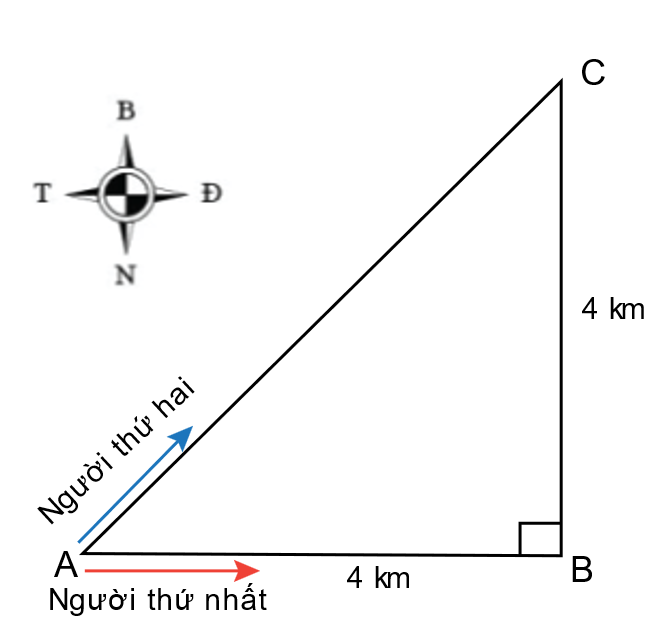
\includegraphics[width=0.5\linewidth]{figs/VN10-2022-PH-TP004-P-3}
	}
	\loigiai{}
	
\end{ex}
% ===================================================================
\begin{ex}
	Khi nhìn vào tốc kế của ô tô đang chạy, số chỉ trên tốc kế cho ta biết
	\choice
	{gia tốc tức thời của ô tô}
	{vận tốc tức thời của ô tô}
	{\True tốc độ tức thời của ô tô}
	{tốc độ trung bình của ô tô}
	\loigiai{}
\end{ex}
% ===================================================================
\begin{ex}
	Một máy bay phản lực có tốc độ $\SI{700}{\kilo\meter/\hour}$. Nếu muốn bay liên tục trên khoảng cách $\SI{1400}{\kilo\meter}$ thì máy bay phải bay trong thời gian là
	\choice
	{\True $\SI{2}{\hour}$}
	{$\SI{3}{\hour}$}
	{$\SI{2}{\hour}\SI{30}{\minute}$}
	{$\SI{1}{\hour}\SI{30}{\minute}$}
	\loigiai{Thời gian máy bay bay quãng đường $\SI{1400}{\kilo\meter}$:
		$$t=\dfrac{s}{v}=\SI{2}{\hour}.$$}
\end{ex}
% ===================================================================
\begin{ex}
	Đồ thị độ dịch chuyển – thời gian trong chuyển động thẳng của một chất điểm có dạng như hình vẽ.\\
	Trong thời gian nào xe chuyển động thẳng đều?
	\begin{center}
		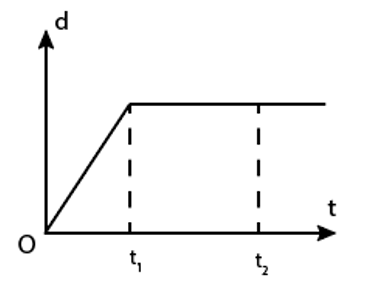
\includegraphics[width=0.25\linewidth]{figs/VN10-2023-PH-TP005-P-4}
	\end{center}
	\choice
	{\True Trong khoảng thời gian từ $0$ đến $t_1$}
	{Trong khoảng thời gian từ $0$ đến $t_2$}
	{Trong khoảng thời gian từ $t_1$ đến $t_2$}
	{Không có lúc nào xe chuyển động thẳng đều}
	\loigiai{}
\end{ex}
% ===================================================================
\begin{ex}
	Phương trình chuyển động của một chất điểm dọc theo trục $Ox$ có dạng: $x = 5 + 60t$ ($x$ đo bằng kilomét và $t$ đo bằng giờ). Chất điểm đó xuất phát từ điểm nào và chuyển động với vận tốc bằng bao nhiêu?
	\choice
	{Từ điểm $O$, với vận tốc $\SI{5}{\kilo\meter/\hour}$}
	{Từ điểm $O$, với vận tốc $\SI{60}{\kilo\meter/\hour}$}
	{Từ điểm cách $O$ $\SI{5}{\kilo\meter/\hour}$, với vận tốc $\SI{5}{\kilo\meter/\hour}$}
	{\True Từ điểm cách $O$ $\SI{5}{\kilo\meter/\hour}$, với vận tốc $\SI{60}{\kilo\meter/\hour}$}
	\loigiai{}
\end{ex}
% ===================================================================
\begin{ex}
Phương trình chuyển động của một chất điểm dọc theo $Ox$ có dạng: $x=5t-12$ (km), với $t$ đo bằng giờ. Độ dịch chuyển của chất điểm từ $\SI{2}{\hour}$ đến $\SI{4}{\hour}$ là	
	\choice
	{$\SI{8}{\kilo\meter}$}
	{$\SI{6}{\kilo\meter}$}
	{\True $\SI{10}{\kilo\meter}$}
	{$\SI{2}{\kilo\meter}$}
	\loigiai{}
\end{ex}
% ===================================================================
\begin{ex}
	Phương trình chuyển động của một chất điểm dọc theo trục $Ox$ có dạng: $x = 4 -10t$ ($x$ đo bằng kilomét và $t$ đo bằng giờ). Quãng đường đi được của chất điểm sau $\SI{2}{\hour}$ chuyển động là
	\choice
	{$\SI{-20}{\kilo\meter}$}
	{\True $\SI{20}{\kilo\meter}$}
	{$\SI{-8}{\kilo\meter}$}
	{$\SI{8}{\kilo\meter}$}
	\loigiai{}
\end{ex}

% ===================================================================
\begin{ex}
	Một xe xuất phát từ lúc 7 giờ 15 phút sáng từ thành phố M, chuyển động thẳng đều tới thành phố N, cách thành phố M $\SI{90}{\kilo\meter}$. Biết tốc độ của xe là $\SI{60}{\kilo\meter/\hour}$, xe đến thành phố N lúc
	\choice
	{9 giờ 45 phút}
	{8 giờ 30 phút}
	{9 giờ 30 phút}
	{\True 8 giờ 45 phút}
	\loigiai{Thời gian để xe đi từ M đến N:
		$$\Delta t=\dfrac{s}{v}=\SI{1.5}{\hour}.$$
		Thời điểm xe đến N:
		$$t=\SI{7}{\hour}\SI{15}{\minute}+\Delta t=\SI{8}{\hour}\SI{45}{\minute}.$$}
\end{ex}
% ===================================================================
\begin{ex}
	Trong nội dung thi đấu môn bơi ếch $\SI{100}{\meter}$, một vận động viên đã hoàn thành đường đua với thành tích $\SI{63.25}{\second}$. Tốc độ trung bình của vận động viên này trong giải thi đấu đó là bao nhiêu?
	\choice
	{\True $\SI{1.58}{\meter/\second}$}
	{$\SI{0.63}{\meter/\second}$}
	{$\SI{6.33}{\meter/\second}$}
	{$\SI{36.75}{\meter/\second}$}
	\loigiai{ Tốc độ trung bình của vận động viên này
		$$v_\text{tb}=\dfrac{s}{t}\approx\SI{1.58}{\meter/\second}.$$}
\end{ex}
% ===================================================================
\begin{ex}
Một ô tô chạy thử nghiệm trên một đoạn đường thẳng. Cứ $\SI{5}{\second}$ thì có một giọt dầu từ động cơ của ô tô rơi thẳng xuống mặt đường. Hình bên cho thấy mô hình các giọt dầu để lại trên mặt đường. Ô tô chuyển động trên đường này với tốc độ trung bình là
\begin{center}
	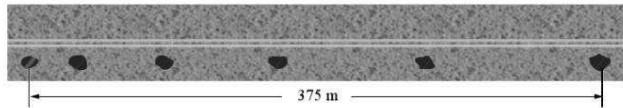
\includegraphics[width=0.5\linewidth]{figs/VN10-2022-PH-TP004-1-P-1}
\end{center}	
	\choice
	{$\SI{12.5}{\meter/\second}$}
	{\True $\SI{15}{\meter/\second}$}
	{$\SI{30}{\meter/\second}$}
	{$\SI{25}{\meter/\second}$}
	\loigiai{Tốc độ trung bình của ô tô:
		$$v_\text{tb}=\dfrac{s}{t}=\dfrac{\SI{375}{\meter}}{\SI{25}{\second}}=\SI{15}{\meter/\second}.$$}
\end{ex}
% ===================================================================
\begin{ex}
	Một xe chuyển động thẳng không đổi chiều, $\SI{1}{\hour}$ đầu xe chạy với tốc độ trung bình $\SI{60}{\kilo\meter/\hour}$ và $\SI{3}{\hour}$ sau xe chạy với tốc độ trung bình $\SI{40}{\kilo\meter/\hour}$. Tốc độ trung bình của xe trong suốt thời gian chuyển động là
	\choice
	{$\SI{48}{\kilo\meter/\hour}$}
	{$\SI{40}{\kilo\meter/\hour}$}
	{$\SI{58}{\kilo\meter/\hour}$}
	{\True $\SI{45}{\kilo\meter/\hour}$}
	\loigiai{$$v_{tb}=\dfrac{v_1t_1+v_2t_2}{t_1+t_2}=\SI{45}{\kilo\meter/\hour}.$$}
\end{ex}
% ===================================================================
\begin{ex}
	Một người đi xe đạp trên $\dfrac{2}{3}$ đoạn đường đầu với tốc độ trung bình $\SI{10}{\kilo\meter/\hour}$ và $\dfrac{1}{3}$ đoạn đường sau với tốc độ trung bình $\SI{20}{\kilo\meter/\hour}$. Tốc độ trung bình của người đi xe đạp trên cả quãng đường là
	\choice
	{\True $\SI{12}{\kilo\meter/\hour}$}
	{$\SI{15}{\kilo\meter/\hour}$}
	{$\SI{17}{\kilo\meter/\hour}$}
	{$\SI{13.3}{\kilo\meter/\hour}$}
	\loigiai{Gọi $s$ là chiều dài đoạn đường
		$$v_{tb}=\dfrac{s}{t_1+t_2}=\dfrac{s}{\dfrac{2s}{3v_1}+\dfrac{s}{3v_2}}=\dfrac{1}{\dfrac{2}{3v_1}+\dfrac{1}{3v_2}}=\SI{12}{\kilo\meter/\hour}.$$}
\end{ex}
% ===================================================================
\begin{ex}
	Hình vẽ bên là đồ thị độ dịch chuyển - thời gian của một chiếc xe ô tô chạy từ $A$ đến $B$ trên một đường thẳng. Vận tốc của xe bằng
\begin{center}
	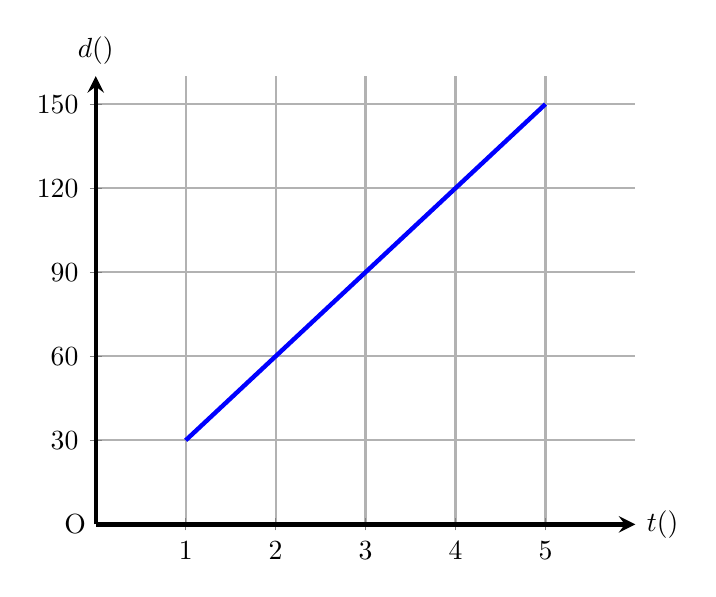
\begin{tikzpicture}  
		\begin{axis}[  ultra thick,
			xmin=0,  
			xmax=6,  
			xtick={0,1,...,5},
			ytick={0,30,...,150},
			minor x tick num=0,
			minor y tick num=0,
			ymin=0,  
			ymax=160, 
			samples=300,
			axis lines=center, 
			grid style={step=1, line width =0.4pt, color=gray!30!white},
			grid=both,
			major grid style={line width=0.8pt,gray!60!white},
			xlabel=$\xsi{t}{\left(\si{\hour}\right)}$, 		ylabel=$\xsi{d}{\left(\si{\kilo\meter}\right)}$,
			every axis y label/.style={at=(current axis.above origin),anchor=south},  
			every axis x label/.style={at=(current axis.right of origin),anchor=west},  ]
			\addplot [ultra thick, blue, smooth, domain=1:5] {30*x};			 
		\end{axis}  
		\node[left] at (0,0) {O};
	\end{tikzpicture}
\end{center}
	\choice
	{\True $\SI{30}{\kilo\meter/\hour}$}
	{$\SI{150}{\kilo\meter/\hour}$}
	{$\SI{120}{\kilo\meter/\hour}$}
	{$\SI{100}{\kilo\meter/\hour}$}
	\loigiai{}
\end{ex}
% ===================================================================
\begin{ex}
Một chất điểm chuyển động trên một đường thẳng. Đồ thị độ dịch chuyển theo thời gian của chất điểm được mô tả như hình vẽ. Tốc độ trung bình của chất điểm trong khoảng thời gian từ 0 đến $\SI{5}{\second}$ là
	\begin{center}
		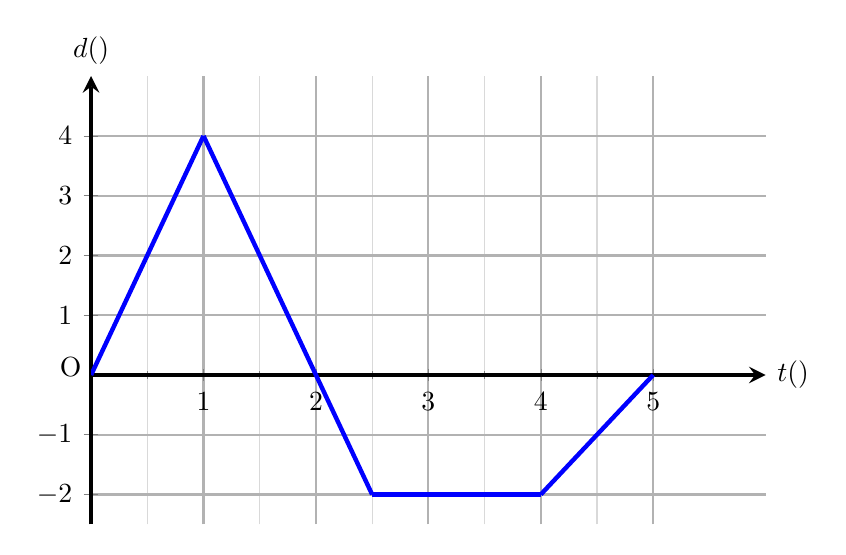
\begin{tikzpicture}  
			\begin{axis}[  ultra thick,xscale=1.25,
				xmin=0,  
				xmax=6,  
				xtick={0,1,...,5},
				ytick={-2,-1,0,1,...,4},
				minor x tick num=1,
				minor y tick num=0,
				ymin=-2.5,  
				ymax=5, 
				samples=300,
				axis lines=center, 
				grid style={step=1, line width =0.4pt, color=gray!30!white},
				grid=both,
				major grid style={line width=0.8pt,gray!60!white},
				xlabel=$\xsi{t}{\left(\si{\second}\right)}$, 		ylabel=$\xsi{d}{\left(\si{\centi\meter}\right)}$,
				every axis y label/.style={at=(current axis.above origin),anchor=south},  
				every axis x label/.style={at=(current axis.right of origin),anchor=west},  ]
				\addplot [ultra thick, blue, smooth, domain=0:1] {4*x};	
				\addplot [ultra thick, blue, smooth, domain=1:2.5] {4-4*(x-1)};		
				\addplot [ultra thick, blue, smooth, domain=2.5:4] {-2};	 
				\addplot [ultra thick, blue, smooth, domain=4:5] {-2+2*(x-4)};
				
			\end{axis}  
		\node[left] at (0,2) {O};
			
		\end{tikzpicture}
	\end{center}
	\choice
	{$\SI{1.6}{\centi\meter/\second}$}
	{$\SI{6.4}{\centi\meter/\second}$}
	{$\SI{4.8}{\centi\meter/\second}$}
	{\True $\SI{2.4}{\centi\meter/\second}$}
	\loigiai{
Tốc độ trung bình của chất điểm:
$$v_\text{tb}=\dfrac{s}{t}=\dfrac{4+4+2+2}{5}=\SI{2.4}{\centi\meter/\second}.$$	
}
\end{ex}
% ===================================================================
\begin{ex}
	Đồ thị toạ độ - thời gian của hai xe (I) và (II) cùng chuyển động trên một đường thẳng được thể hiện như hình bên. Thời điểm hai xe gặp nhau là
	\begin{center}
		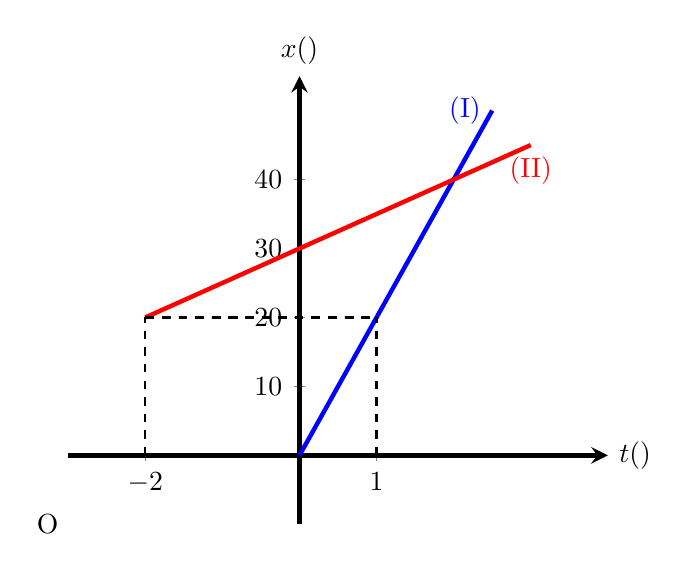
\begin{tikzpicture}  
			\begin{axis}[  ultra thick,
				xmin=-3,  
				xmax=4,  
				xtick={-2,0,1},
				ytick={0,10,...,40},
				minor x tick num=0,
				minor y tick num=0,
				ymin=-10,  
				ymax=55, 
				samples=300,
				axis lines=center, 
				xlabel=$\xsi{t}{\left(\si{\hour}\right)}$, 		ylabel=$\xsi{x}{\left(\si{\kilo\meter}\right)}$,
				every axis y label/.style={at=(current axis.above origin),anchor=south},  
				every axis x label/.style={at=(current axis.right of origin),anchor=west},  ]
				\addplot [ultra thick, blue, smooth, domain=0:2.5] {20*x} node[left] {(I)};	
				\addplot [ultra thick, red, smooth, domain=-2:3] {30+5*x} node[below] {(II)};	
				\addplot [thick, dashed, domain=-2:1] {20} ;	
				\draw[thick, dashed] (axis cs:-2,0) --(axis cs:-2,20);	 
				\draw[thick, dashed] (axis cs:1,0) --(axis cs: 1,20);
			\end{axis}  
			\node[left] at (0,0) {O};
		\end{tikzpicture}
	\end{center}
	\choice
	{$\SI{1}{\hour}$}
	{\True$\SI{2}{\hour}$}
	{$\SI{2.5}{\hour}$}
	{$\SI{1.33}{\hour}$}
	\loigiai{}
\end{ex}

% ===================================================================
\begin{ex}
	Hình dưới là đồ thị độ dịch chuyển - thời gian của hai vật chuyển động thẳng cùng hướng. Tỉ lệ vận tốc $\dfrac{v_A}{v_B}$ là
	\begin{center}
		\begin{tikzpicture} 
			\coordinate (O)  at (0,0);
			\coordinate (t) at (4,0);
			\coordinate (d) at (0,4);
			\coordinate (A) at ($(O)+(30:3)$);
			\coordinate (B) at ($(O)+(60:3.5)$);
			\draw[line width=1pt, -latex] (O)--(d);
			\draw[line width=1pt, -latex] (O)--(t);
			\draw[line width=1.5pt, red] (O)--(A);
			\draw[line width=1.5pt, blue] (O)--(B);
			\node[left] at (O) {O};
			\node[above] at (t) {$t$};
			\node[left] at (d) {$d$};
			\tkzFillAngle[size=0.75cm,color=red, fill=red, opacity=0.25](t,O,A);
			\tkzLabelAngle[color=red,pos=1.2](t,O,A){$\SI{30}{\degree}$}
				\tkzMarkAngle[size=0.5cm,color=blue](t,O,B);
		\node[blue] at (0.75,0.7) {$\SI{60}{\degree}$};
		\end{tikzpicture}
	\end{center}
	\choice
	{$\dfrac{3}{1}$}
	{$\dfrac{1}{3}$}
	{$\dfrac{\sqrt{3}}{1}$}
	{$\dfrac{1}{\sqrt{3}}$}
	\loigiai{}
\end{ex}


\Closesolutionfile{ans}
\begin{center}
	\textbf{--- HẾT ---}
\end{center}